\documentclass{standalone}
\usepackage{tikz}
\usepackage{amsmath}
\usepackage{graphicx}
\usetikzlibrary{positioning, shapes.geometric, shapes.multipart, arrows.meta, calc, fit}

% Global layout controls
\def\mainNodeSep{0.95cm}
\def\rowGap{0.42cm}
\def\colGap{0.9cm}
\def\legendOffsetX{1.2cm}
\def\legendPanelW{14.8cm}
\def\legendPanelH{10.2cm}
\def\legendPadX{0.6cm}
\def\legendTopInset{1.6cm}
\def\legendBottomInset{1.0cm}
\def\curveRound{5pt}

\newcommand{\MMMLSharedStyles}{
  \tikzset{
    basebox/.style={
      rectangle,
      rounded corners=2.5pt,
      draw=black!70,
      minimum height=0.95cm,
      minimum width=2.1cm,
      align=center
    },
    dense/.style={basebox, fill=orange!25,  minimum height=1.0cm, minimum width=1.2cm, text width=1.9cm},
    process/.style={dense},
    process2/.style={basebox, fill=orange!15, minimum height=0.8cm, text width=3.9cm},
    silu/.style={
      circle, draw=black!70, fill=white, minimum size=1.0cm,
      path picture={
        \draw[-, line width=0.9pt] (path picture bounding box.center) circle (0.28cm);
        \begin{scope}
          \clip (path picture bounding box.center) circle (0.28cm);
          \draw[-, domain=-2:2,smooth,variable=\x,line width=0.7pt]
            plot ({0.11*\x},{0.11*(\x/(1+exp(-\x)))});
        \end{scope}
      }
    },
    plusop/.style={
      circle, draw=black!70, fill=white, minimum size=1cm,
      path picture={
        \draw[-, line width=0.9pt]
          (path picture bounding box.west) -- (path picture bounding box.east);
        \draw[-, line width=0.9pt]
          (path picture bounding box.south) -- (path picture bounding box.north);
      }
    },
    basis/.style={basebox, fill=cyan!25, minimum height=1.0cm, minimum width=3.2cm},
    message/.style={basebox, fill=green!30, minimum height=1.2cm, minimum width=4.2cm},
    tensor/.style={basebox, fill=red!25, minimum height=1.2cm, minimum width=2.2cm},
    extra/.style={basebox, fill=gray!25, minimum height=1.2cm, minimum width=2.2cm},
    embedding/.style={basebox, fill=blue!25, minimum height=1.2cm, minimum width=4.2cm},
    output/.style={basebox, fill=yellow!25, minimum height=0.95cm, minimum width=0.8cm, align=center, font=\sffamily\Large},
    legendbox/.style={rectangle, draw=black!60, rounded corners=1.5pt, minimum width=0.8cm, minimum height=0.55cm},
    legendtext/.style={anchor=west, font=\sffamily\Large, align=left, text width=12.8cm}
  }
}


\begin{document}
\resizebox{\textwidth}{!}{%
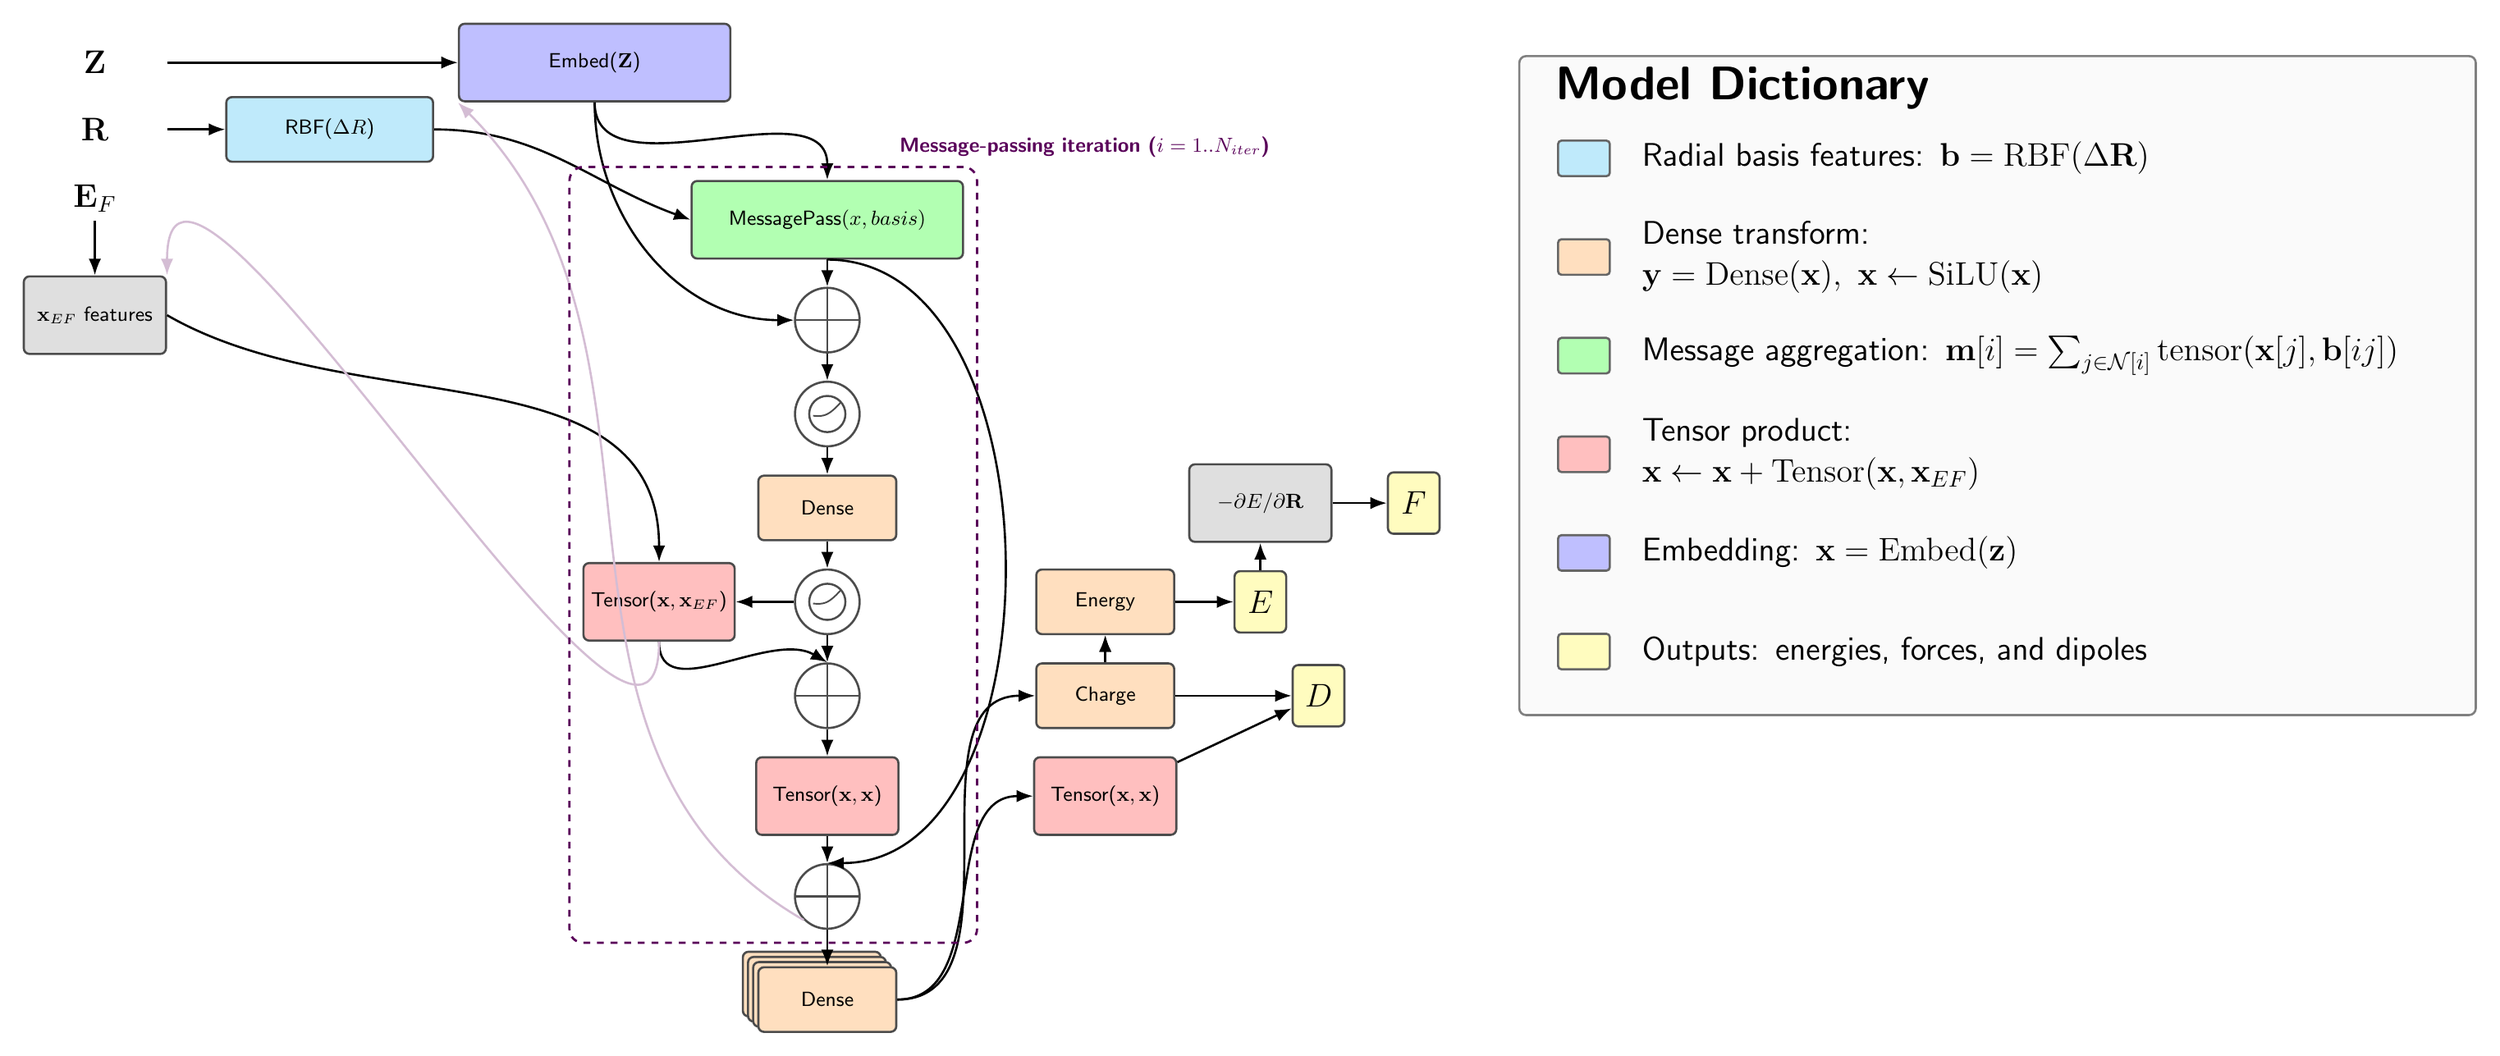
\begin{tikzpicture}[
  auto,
  node distance=\mainNodeSep and \mainNodeSep,
  line width=0.95pt,
  >=Latex,
  ->,
  font=\sffamily\small
]
  \MMMLSharedStyles

  % Inputs
  \node[minimum width=2.2cm, font=\sffamily\Large] (zin) {$\mathbf{Z}$};
  \node[minimum width=2.2cm, below=\rowGap of zin, font=\sffamily\Large] (rin) {$\mathbf{R}$};
  \node[minimum width=2.2cm, below=\rowGap of rin, font=\sffamily\Large] (efin) {$\mathbf{E}_F$};

  % Feature construction
  \node[embedding, right=5*\colGap of zin] (embed) {Embed($\mathbf{Z}$)};
  \node[basis, right=\colGap of rin] (basis) {RBF($\Delta R$)};
  \node[extra, below=2*\rowGap of efin] (efbuild) {$\mathbf{x}_{EF}$ features};
%   \node[basebox, fill=white, right=\colGap of efbuild, minimum width=2.2cm] (xtype) {$x_{EF}^{(\ell\le \ell_{\max})}$};
\draw[->] (efin) -- (efbuild);
  \draw[->] (zin) -- (embed);
  \draw[->] (rin) -- (basis);
%   \draw[->] (efin) -- (efbuild);
%   \draw[->] (efbuild) -- (xtype) node[midway, above, font=\scriptsize] {$\ell\le \ell_{\max}$};

  % Message passing iteration core
  \node[message, below=1.2cm of embed, xshift=4*\colGap] (msg) {MessagePass$(x,basis)$};
  \node[plusop, below=\rowGap of msg] (sum1) {};
  \node[silu, below=\rowGap of sum1] (silu1) {};
  \node[dense, below=\rowGap of silu1] (dense1) {Dense};
  \node[silu, below=\rowGap of dense1] (silu2) {};
  \node[tensor, left=\colGap of silu2] (tensor) {Tensor($\mathbf{x},\mathbf{x}_{EF}$)};
  \node[plusop, below=\rowGap of silu2] (sum2) {};
  \node[tensor, below=\rowGap of sum2] (tdense) {Tensor($\mathbf{x},\mathbf{x}$)};
  \node[plusop, below=\rowGap of tdense] (sum3) {};
  \coordinate (stackbase) at ($(sum3)+(0,-3.8*\rowGap)$);
  \node[dense] (stack1) at ($(stackbase)+(-0.24,0.24)$) {Dense};
  \node[dense] (stack2) at ($(stackbase)+(-0.16,0.16)$) {Dense};
  \node[dense] (stack3) at ($(stackbase)+(-0.08,0.08)$) {Dense};
  \node[dense] (stack4) at (stackbase) {Dense};

  \draw[->] (embed.south) to[out=-90,in=90] (msg.north);
  \draw[->] (basis.east) to[out=0,in=160] (msg.west);
  \draw[->] (msg.south) to[out=-90,in=90] (sum1.north);
  \draw[->] (embed.south) to[out=-90,in=180] (sum1.west);
  \draw[->] (sum1) -- (silu1);
  \draw[->] (tensor.south) to[out=-90,in=150] (sum2.north);
  \draw[->] (silu1) -- (dense1);
  \draw[->] (dense1) -- (silu2);
  \draw[->] (silu2.west) -- (tensor.east);
  \draw[->] (efbuild.east) to[out=-30,in=90] (tensor.north);
%   \draw[->] (tensor.west) to[out=180,in=0] (sum2.west);
  \draw[->] (silu2) -- (sum2);
  \draw[->] (sum2) -- (tdense);
  \draw[->] (tdense) -- (sum3);
  \draw[->] (msg.south) to[out=0,in=0] (sum3.north);
  \draw[->] (sum3) -- (stack4.north);
  \draw[->, color=violet!70!black!26] (sum3.south west) to[out=150,in=-45] (embed.south west);
  \draw[->, color=violet!70!black!26] (tensor.south) to[out=-90,in=90] (efbuild.north east);
%   \draw[->] (sum3.west) to[out=200,in=-70] (embed.south) node[midway, left, font=\scriptsize] {update $\mathbf{x}$};
%   \draw[->] (sum2.west) to[out=170,in=-20] (efbuild.south) node[midway, left, font=\scriptsize] {update $\mathbf{x}_{EF}$};
%   \draw[->] (msg.east) to[out=10,in=-170] (sum1.east); % residual add x+y

  % Output heads
  \node[dense, right=3*\colGap of sum2] (qhead) {Charge};
  \node[dense, above=\rowGap of qhead] (ehead) {Energy};
  \node[tensor, below=\rowGap of qhead] (dhead) {Tensor($\mathbf{x},\mathbf{x}$)};
  \node[output, right=\colGap of ehead] (energy) {$E$};
  \node[output, right=2*\colGap of qhead] (dipole) {$D$};

  \node[extra, above=\rowGap of energy] (dEdR) {$-\partial E/\partial \mathbf{R}$};
  \node[output, right=2*\rowGap of dEdR] (F) {$F$};
    \draw[->] (dEdR) -- (F);
    \draw[->] (energy) -- (dEdR);
    \draw[->] (ehead) -- (energy);

\draw[->] (stack4.east) to[out=0,in=180] (qhead);
\draw[->] (qhead) -- (ehead);
\draw[->] (qhead) -- (ehead);
\draw[->] (stack4.east) to[out=0,in=180] (dhead);
\draw[->] (qhead) -- (dipole);
\draw[->] (dhead) -- (dipole);

  \node[draw=violet!70!black, rounded corners=6pt, dashed, line width=1.0pt, inner sep=0.2cm,
    fit=(msg) (sum1) (silu1) (dense1) (silu2) (tensor) (sum2) (tdense) (sum3)] (loop) {};
  \node[anchor=south west, font=\sffamily\small\bfseries, text=violet!70!black] at ($(loop.north east)+(-1.35,0)$) {Message-passing iteration ($i=1..N_{iter}$)};

  \path (current bounding box.north east) coordinate (figNE);
  \node[draw=black!50, rounded corners=3pt, fill=black!2, minimum width=\legendPanelW, minimum height=\legendPanelH, anchor=north west]
    (legendpanel) at ($(figNE)+(\legendOffsetX,0)-(0,0.5)$) {};
  \coordinate (legStart) at ($(legendpanel.north west)+(\legendPadX,-\legendTopInset)$);
  \coordinate (legEnd) at ($(legendpanel.south west)+(\legendPadX,\legendBottomInset)$);
  \coordinate (leg2) at ($(legStart)!0.2!(legEnd)$);
  \coordinate (leg3) at ($(legStart)!0.4!(legEnd)$);
  \coordinate (leg4) at ($(legStart)!0.6!(legEnd)$);
  \coordinate (leg5) at ($(legStart)!0.8!(legEnd)$);

  \node[anchor=north west, font=\sffamily\bfseries\huge] (legendtitle) at ($(legendpanel.north west)+(0.45,-0.05)$) {Model Dictionary};
  \node[legendbox, fill=cyan!25, anchor=west] (lg1) at (legStart) {};
  \node[legendtext, right=0.35cm of lg1.east, anchor=west] {Radial basis features: $\mathbf{b}=\mathrm{RBF}(\Delta\mathbf{R})$};
  \node[legendbox, fill=orange!25, anchor=west] (lg2) at (leg2) {};
  \node[legendtext, right=0.35cm of lg2.east, anchor=west] {Dense transform:\\$\mathbf{y}=\mathrm{Dense}(\mathbf{x}),\ \mathbf{x}\leftarrow\mathrm{SiLU}(\mathbf{x})$};
  \node[legendbox, fill=green!30, anchor=west] (lg3) at (leg3) {};
  \node[legendtext, right=0.35cm of lg3.east, anchor=west] {Message aggregation: $\mathbf{m}[i]=\sum_{j\in\mathcal{N}[i]}\mathrm{tensor}(\mathbf{x}[j],\mathbf{b}[ij])$};
  \node[legendbox, fill=red!25, anchor=west] (lg4) at (leg4) {};
  \node[legendtext, right=0.35cm of lg4.east, anchor=west] {Tensor product:\\$\mathbf{x}\leftarrow\mathbf{x}+\mathrm{Tensor}(\mathbf{x},\mathbf{x}_{EF})$};
  \node[legendbox, fill=blue!25, anchor=west] (lg5) at (leg5) {};
  \node[legendtext, right=0.35cm of lg5.east, anchor=west] {Embedding: $\mathbf{x}=\mathrm{Embed}(\mathbf{z})$};
  \node[legendbox, fill=yellow!25, anchor=west] (lg6) at (legEnd) {};
  \node[legendtext, right=0.35cm of lg6.east, anchor=west] {Outputs: energies, forces, and dipoles};
\end{tikzpicture}%
}
\end{document}
